\section{Classical RIMs in a Dynamic PRA Context}
\label{sec:classicalRIMs_RISMC}

In a Dynamic PRA environment, $R_0$ is obtained (e.g., through Monte-Carlo sampling) by:
\begin{enumerate}
  \item Running $N$ simulation (e.g., RELAP5 runs)
  \item Counting the number $N_{CD}$ of simulations that lead to core damage (CD) condition
  \item Calculating $R_0= \frac{N_CD}{N}$
\end{enumerate}
Note that while basic events in classical PRA are mainly Boolean, in a Dynamic PRA environment the 
sample parameters can be, not only Boolean, but more often continuous. As an example, let consider
two basic events:
\begin{itemize}
  \item Emergency Diesel Generator (EDG) failure to start, and, 
  \item EDG failure to run
\end{itemize}

In classical PRA analyses, a probability value is associated to each basic event. On the other side, 
in a Dynamic PRA framework, a Bernoulli distribution could be associated to the first basic event and 
a continuous distribution (e.g., exponential distribution) could be associated to the second basic event. 
At this point a challenge arises: the determination of $R_i^-$ and $R_i^+$ for each sampled parameter; 
two possible approaches can be followed :
\begin{enumerate}
  \item Perform a Dynamic PRA for $R_0$ and each $R_i^-$ and $R_i^+$
  \item Determine an approximated value of $R_i^-$ and $R_i^+$ from the simulation runs generated to calculate $R_0$
\end{enumerate}
Regarding Approach 1, given the computational costs of each Dynamic PRA, it is unfeasible to determine 
$R_i^-$ and $R_i^+$ for each sampled parameter. In fact, if we consider $M$ sample
parameters (i.e., $S$ basic events), then the risk importance analysis would require $2S+1$ Dynamic PRA analyses.

Regarding Approach 2, a method (implemented in RAVEN as an internal post-processor) was developed and it is 
here presented. This method requires an input from the user:
\begin{itemize}
  \item Range, $I_i^-$, of the variable $s_i$ that can be associated to ``basic event with component perfectly reliable''
  \item Range, $I_i^+$, of the variable $s_i$ that can be associated to ``basic event in a failed status''
\end{itemize}
Given this kind of information, it is possible to calculate $R_i^+$ and $R_i^-$ as follows:
\begin{align} 
  R_0   &= \frac{N_{CD}}{N}  \\
  R_i^+ &= \frac{N_{CD, s_i \in I_i^+}}{N}   \\
  R_i^- &= \frac{N_{CD, s_i \in I_i^-}}{N} 
\end{align}
where:
\begin{itemize}
  \item $N_{CD, s_i \in I_i^+}$ is the number of simulations leading to core damage and with parameter $s_i \in I_i^+$
  \item $N_{CD, s_i \in I_i^-}$ is the number of simulations leading to core damage and with parameter $s_i \in I_i^-$
\end{itemize}

Note that this approach has an issue related to the choices of $I_i^+$ and $I_i^-$. 
Depending on their values, $R_i^+$ and $R_i^-$ might change accordingly. In addition, the statistical error 
associated to the estimates of $R_i^+$ and $R_i^-$ also changes. 
An example is shown in Figure 1 for both cases (discrete and continuous) of a basic event $x_i$ represented 
as a stochastic variable which is sampled (e.g., through a Monte-Carlo process) for each simulation run.
Lets consider the continuous case and assume $s_i$ correspond to the basic event ``EDG failure to run''. 
The user might impose the following in order to determine $R_i^+$ and $R_i^-$:
\begin{itemize}
  \item $I_i^-=[T_i^-,\infty]$ where $T_i^-$ may be set equal to the simulation mission time (e.g., 24 hours). 
        This implies that a sampled value for EDG failure to run greater than 24 hours implies that the 
        EDG actually does not fail to run (reliability equal to 1.0)
  \item $I_i^+=[0,T_i^+ ]$ where $T_i^-$ may be set to an arbitrary small value (e.g., 5 min). This implies that 
        a sampled value for EDG failure to run smaller than 5 min implies a reliability equal to 0.0
\end{itemize}

Note that while the definition of $I_i^-$ is perfectly reasonable, one would argue that a smaller interval 
should be chosen for $I_i^+$ (e.g., 30 seconds or less). 
Recall that ideally, a value of $s_i=0.0$ should be theoretically chosen (and not an interval); however, 
given the nature of the distribution this is not allowed. Given the nature of the problem, we are bound 
to choose an interval $I_i^+$:
\begin{itemize}
  \item A small interval in the neighbor of $s_i=0.0$ would lead to a value of $R_i^+$ close to the theoretical 
        one. 
        However, the number of actual sampled values falling in $I_i^+$ would be very small, i.e., large stochastic 
        error.
  \item A large interval in the neighbor of $s_i=0.0$ would lead to a value of $R_i^+$ far from the theoretical one. 
        However, the number of actual sampled values falling in $I_i^+$ would be very high,
        i.e., small stochastic error.
\end{itemize}

A solution to the large statistical error associated to a very small interval $I_i^+$ can be solved by 
employing different sampling algorithms other than the classical Monte-Carlo one. 
As an example, a better resolution of the final value for $R_i^+$ can be achieved by sampling uniformly 
the range of variability of $x_i$ and associate an importance weight to each sample. At this point
the counting variable $N_{CD}$ is weighted by the weight of each sample. By sampling uniformly the range of 
variability of $x_i$, the number of samples in the interval $I_i^+$ would be significantly higher.

\begin{figure}
    \centering
    \centerline{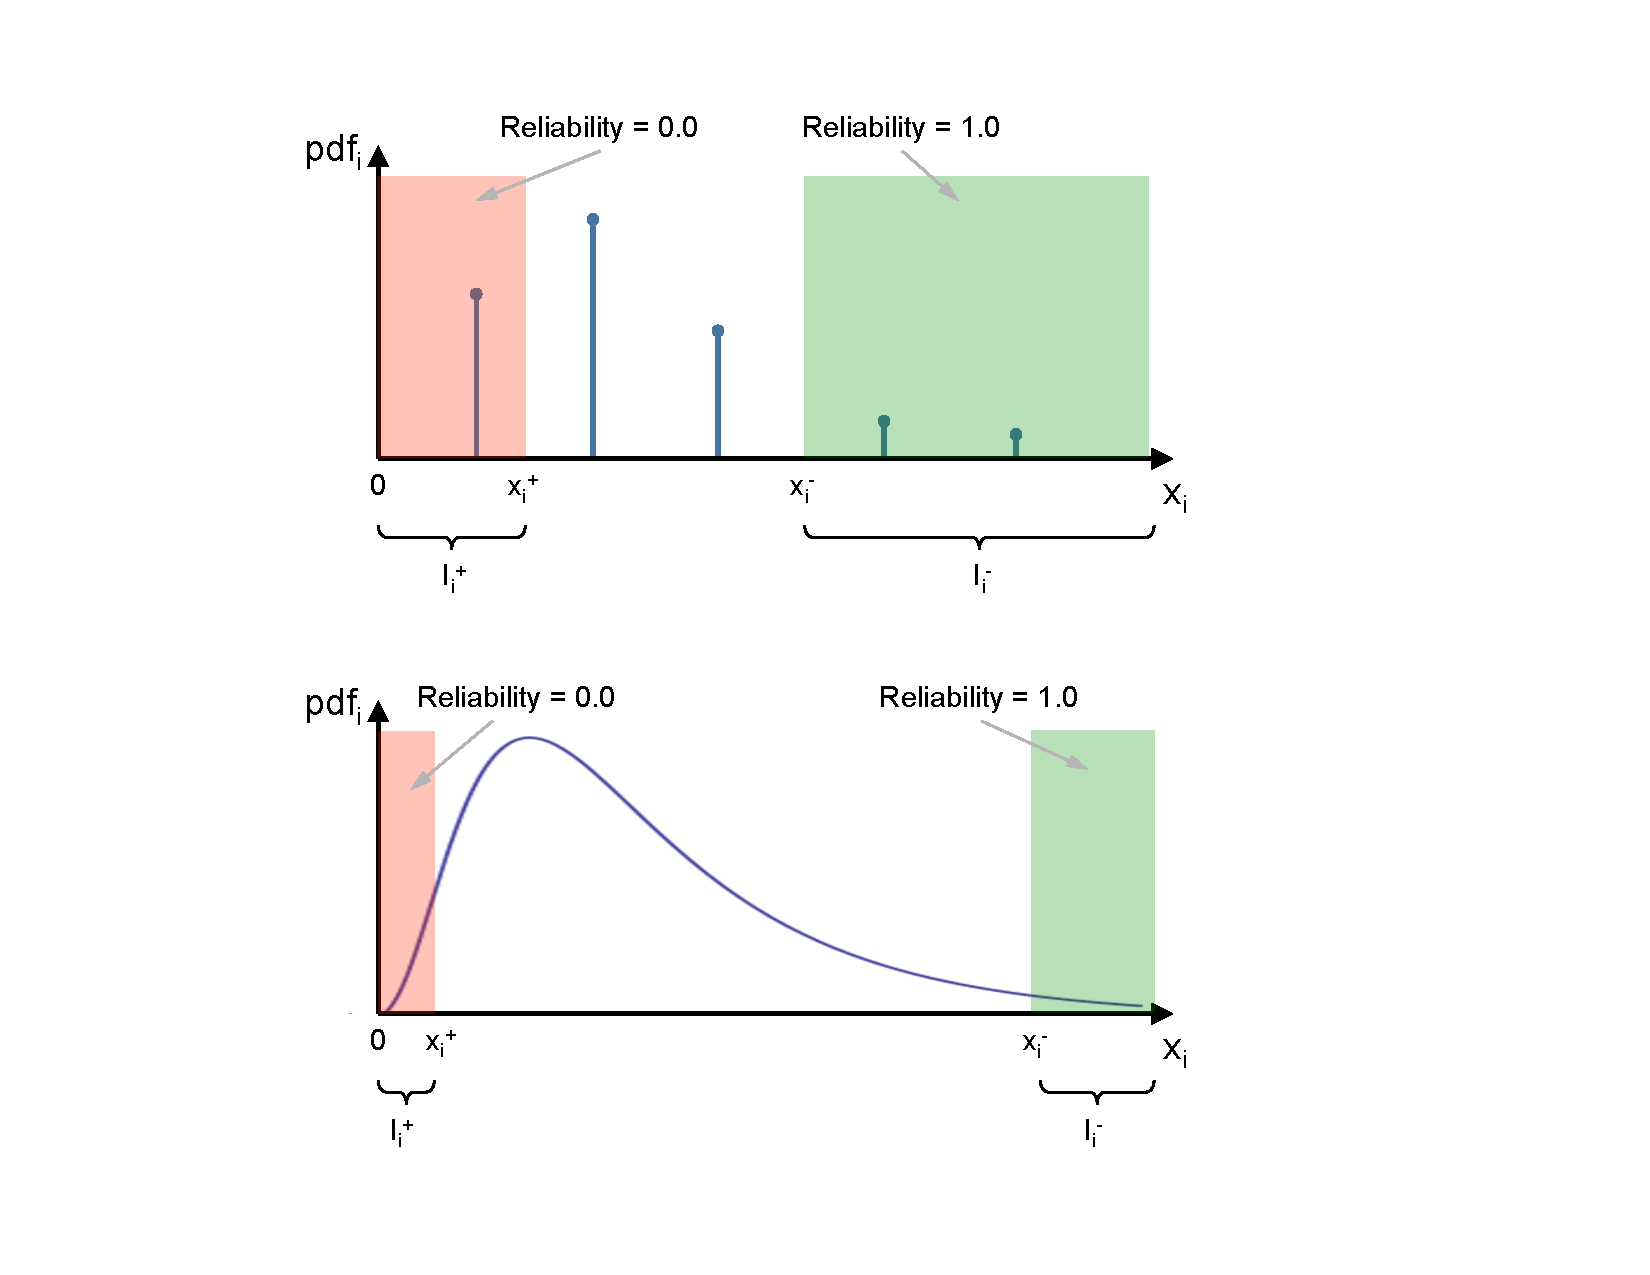
\includegraphics[scale=0.5]{intervals.pdf}} 
    \caption{Treatment of discrete (top) and continuous (bottom) stochastic variables for reliability purposes.}
    \label{fig:intervals}
\end{figure}
